
Nei diagrammi di sequenza viene illustrata la sequenza di operazioni necessarie alla realizzazione degli use case del sistema rispetto agli elementi dell'architettura e alle classi di analisi presenti nel sistema.

Gli use case di HBS possono essere categorizzati, a grandi linee, nelle seguenti categorie:
\begin{itemize}
	\item \emph{transazioni}, per gli use case riguardanti le operazioni che i clienti della banca possono effettuare (incluse le operazioni veloci);

	\item interazioni con il sistema di bidding.
\end{itemize}

\subsubsection{Transazioni}

Gli use case di tipo \emph{transazionale} seguono uno di due modelli:
\begin{itemize}
	\item modello transazionale semplice;

	\item modello transazionale con conferma tramite OTP.
\end{itemize}

In figura~\ref{fig:sequence:transazione:modello} viene indicato il modello transazionale semplice.

\begin{figure*}[h]
	\centering
	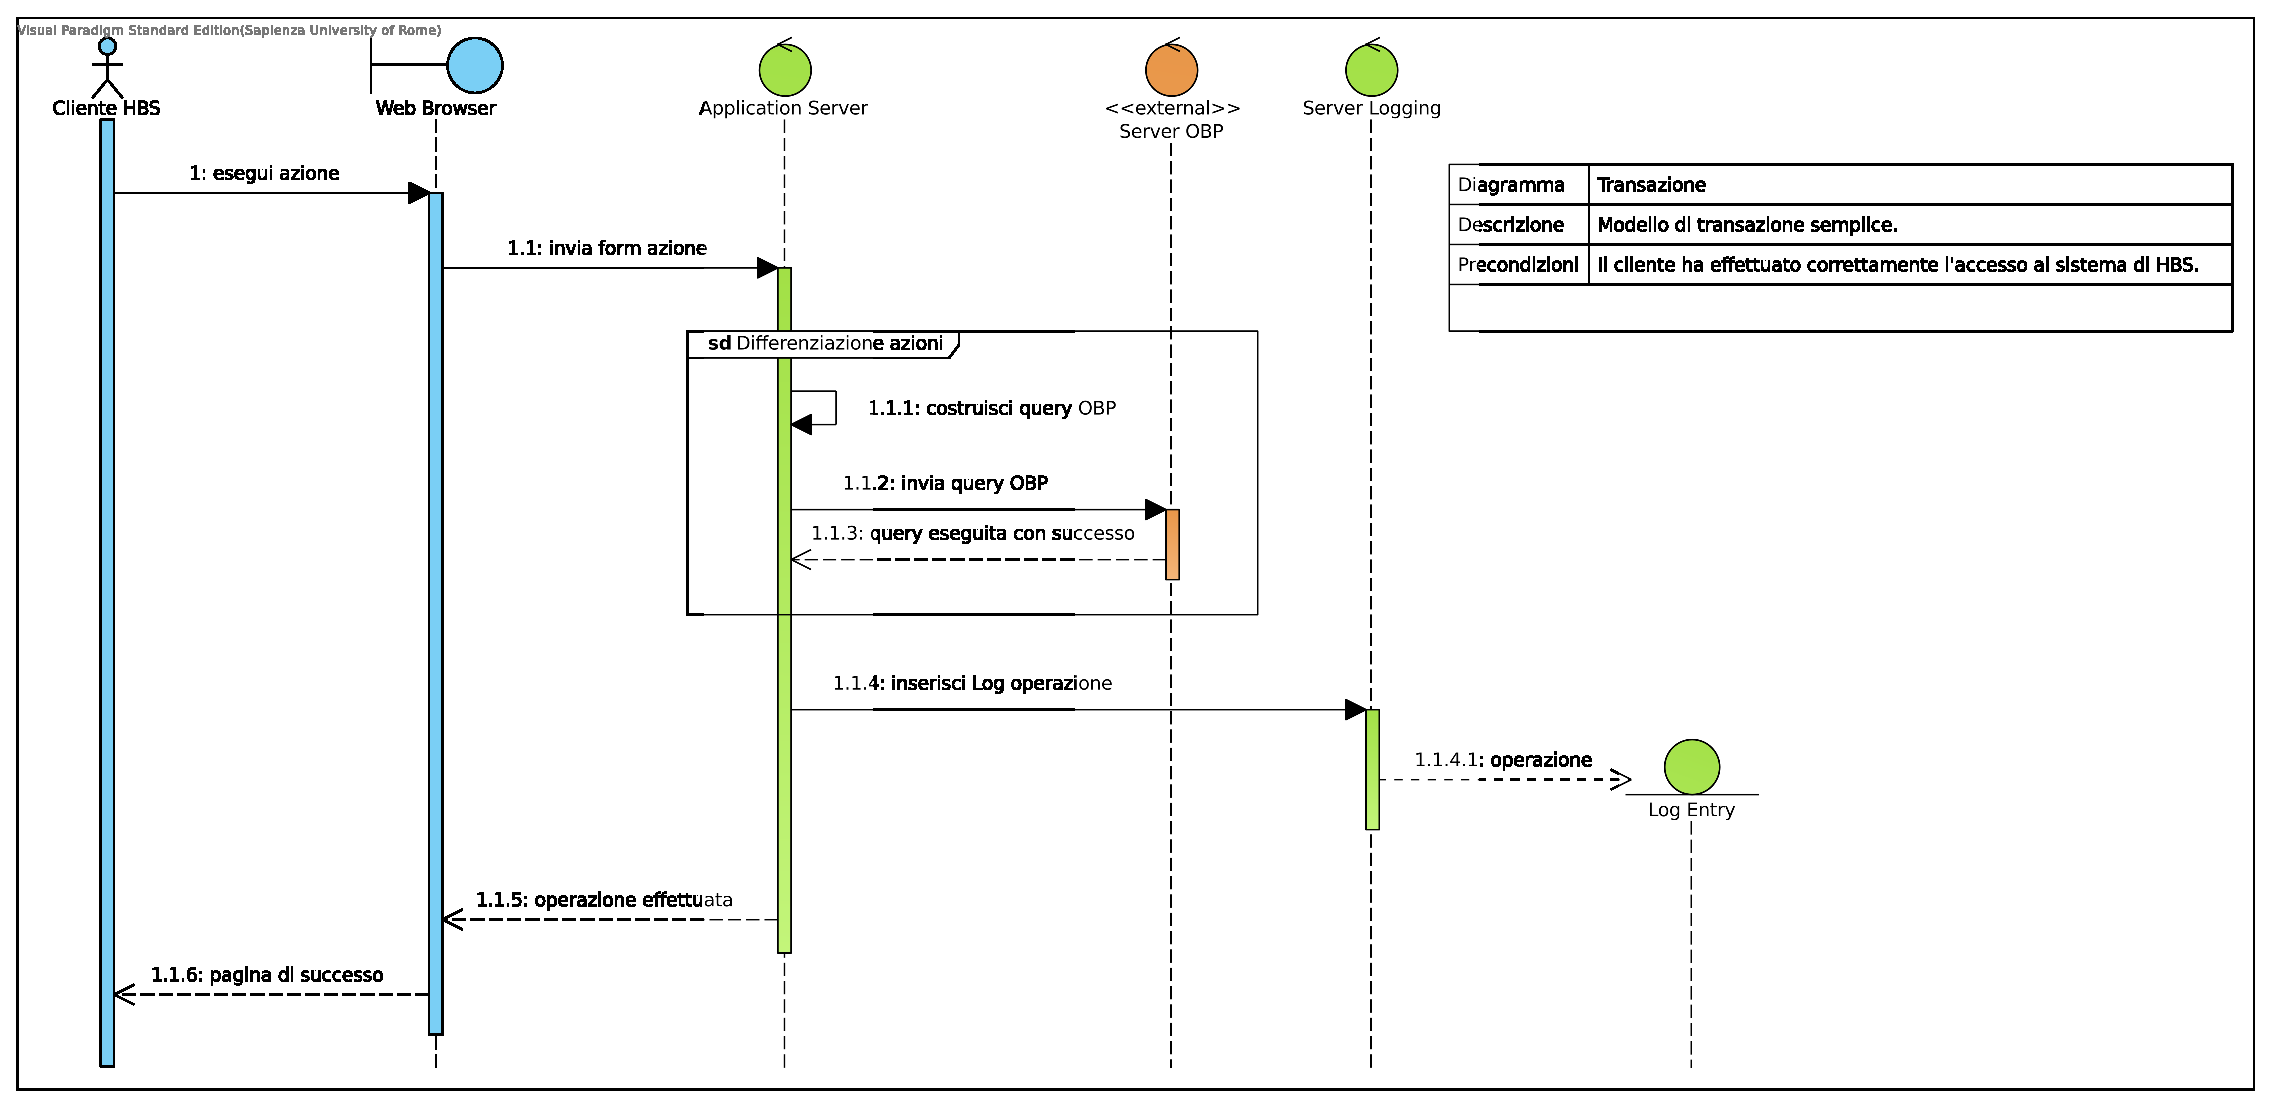
\includegraphics[width=\textwidth]{Images/sequence/Transazione.eps}
	\caption{Modello di transazione semplice.}
	\label{fig:sequence:transazione:modello}
\end{figure*}

In figura~\ref{fig:sequence:transazione-otp:modello} viene indicato il modello transazionale con conferma tramite OTP.
Use case di questo tipo sono, ad esempio, gli use case riguardanti le operazioni effettuabili da un conto bancario.

\begin{figure*}[h]
	\centering
	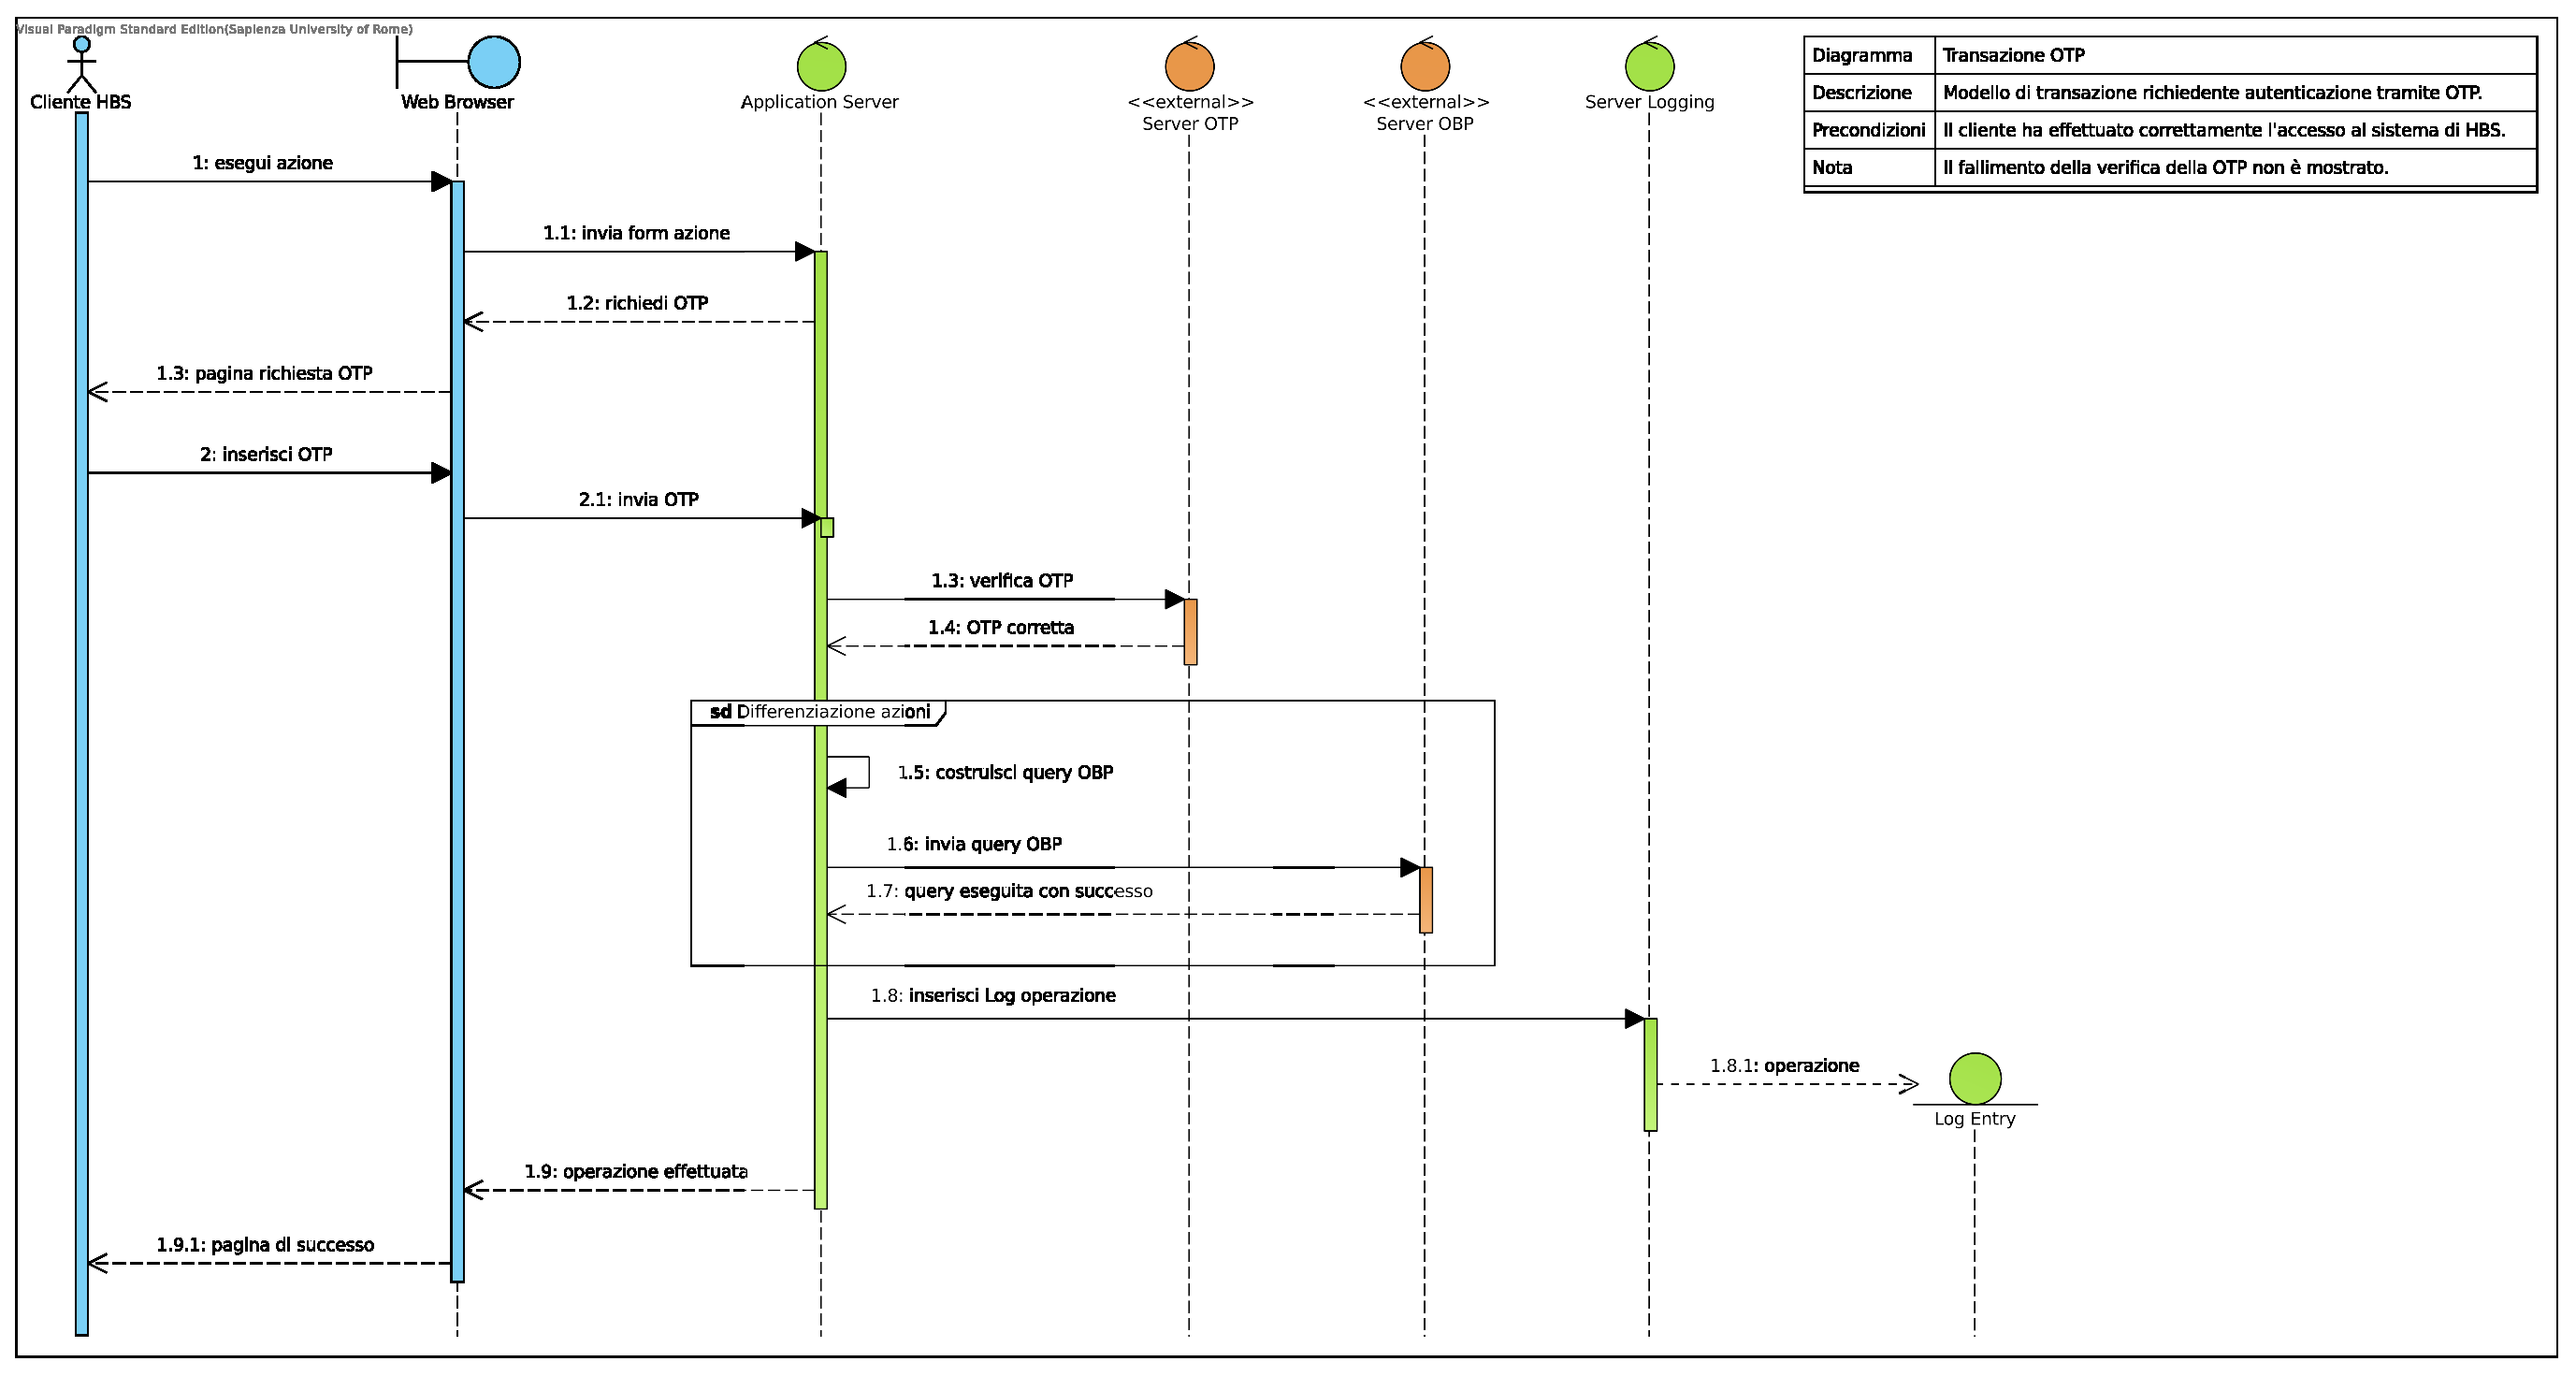
\includegraphics[width=\textwidth]{Images/sequence/Transazione_OTP.eps}
	\caption{Modello di transazione per la quale è richiesta la conferma tramite OTP.}
	\label{fig:sequence:transazione-otp:modello}
\end{figure*}
